\captionsetup{font={scriptsize,sc,up,singlespacing}}
%\begin{figure}[h] % Figure at bottom of the page ([b] argument, could be "t" for top or "h" for here)
%	\centering
%	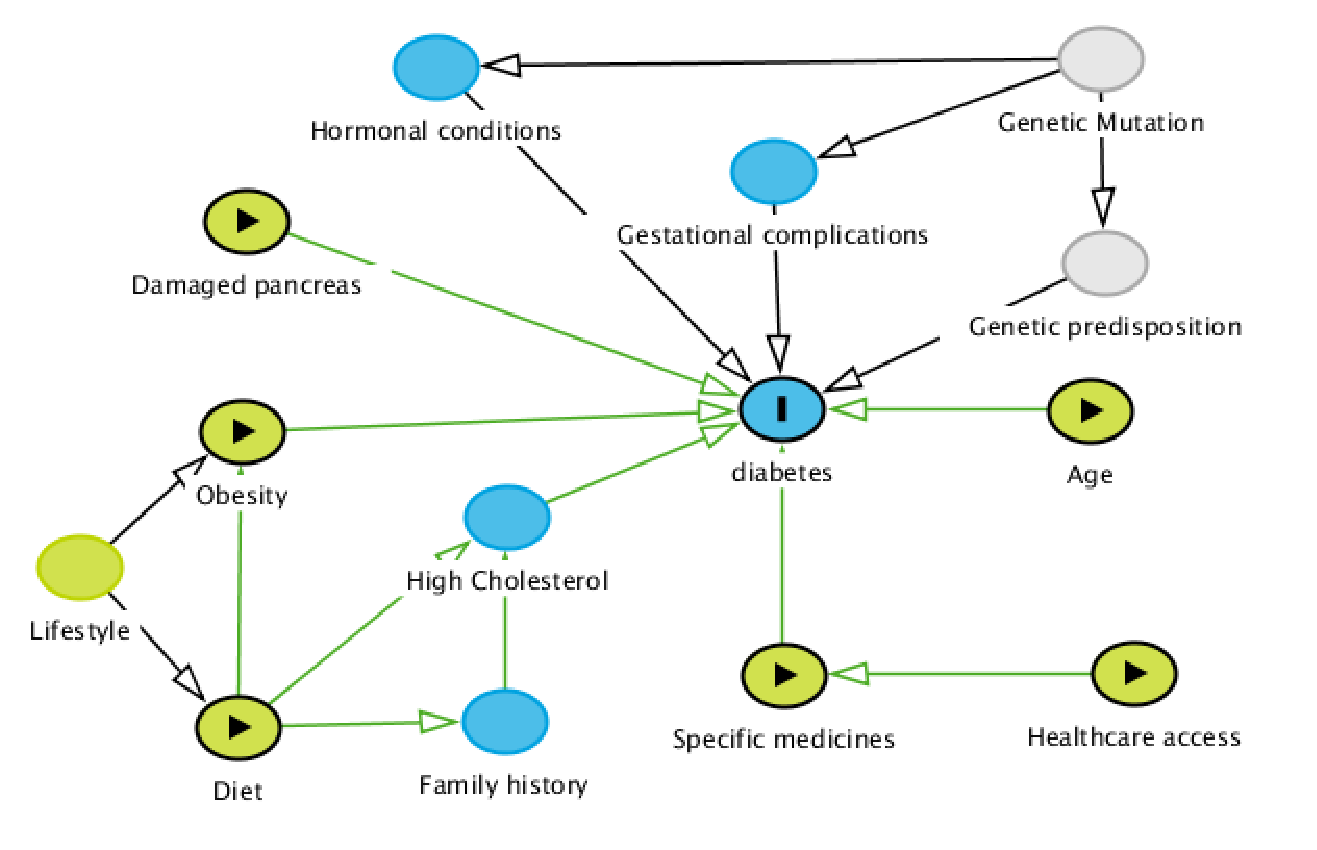
\includegraphics[width=.8\textwidth]{diabetes-causalmodel}
%       \label{fig:diabetes-cm}
%\end{figure}

\begin{figure*}[ht]\centering % Using \begin{figure*} makes the figure take up the entire width of the page
	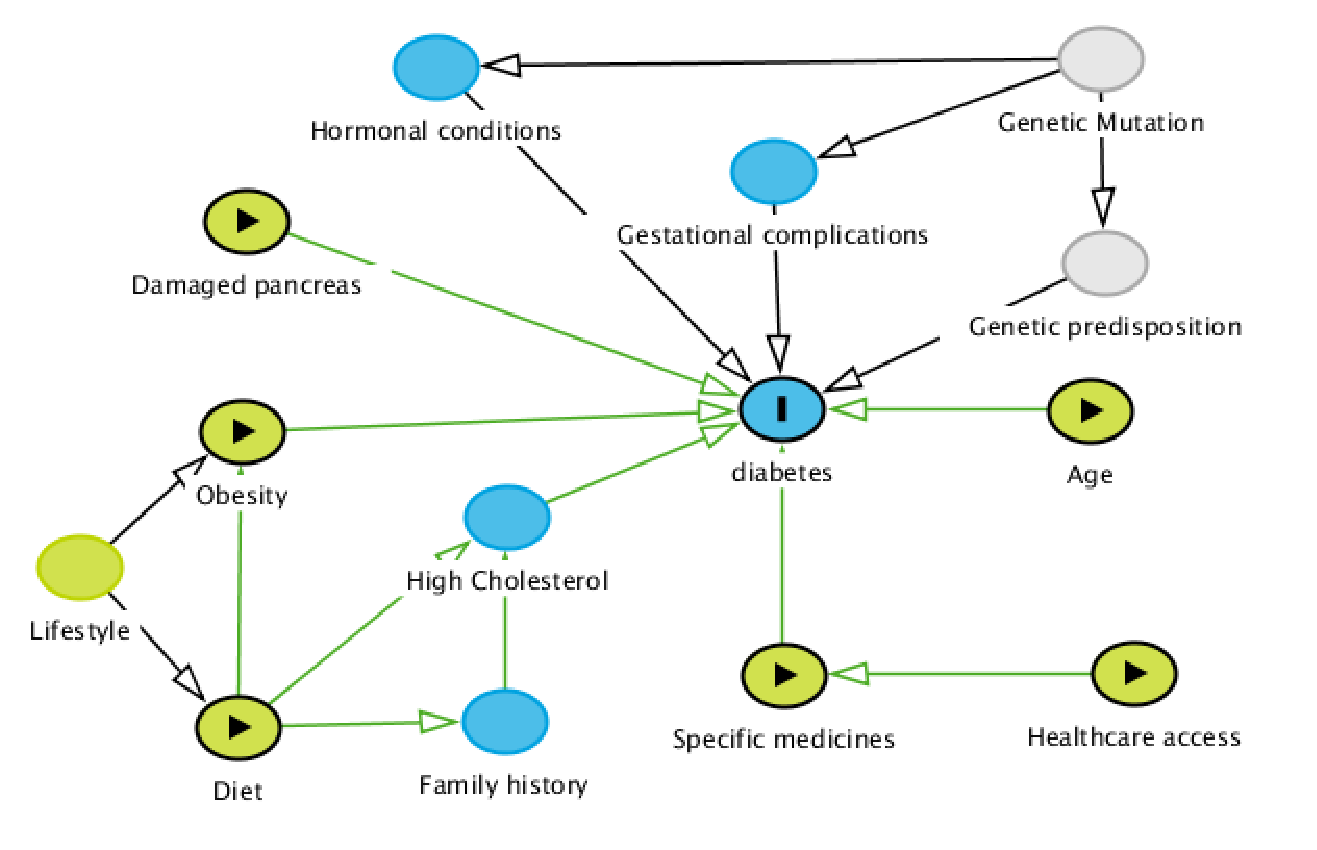
\includegraphics[width=\linewidth]{diabetes-causalmodel.eps}
	\caption{ \textbf{Example of a graphical causal model for diabetes that can be used for probablistic and causal reasoning:}
diabetes is a complex disease where simple GWAS deliver significant SNP hits that do not necessarily lead to new treatments because of confounding factors, including environment and genetic variants that differ between people. This is especially relevant for individuals belonging to minorities.
Some of Shelby Solomon's postdoc research will explore AI-type inferencing mechanisms using Judea Pearl's graphical models for probabilistic and causal reasoning: starting from the existing Bayesian network webserver (BNW) logic that is already in GeneNetwork Shelby Solomon will, in the long-term, add AI-type inferencing mechanisms to see if we can improve scale and logic and expose these tools through the \GN\ user interface.
The goal is to get answers to causal questions about specific health issues, including asthma, sickle cell disease, and epilepsy in the BIG cohort. In \GN\ we will also target gout, diabetes, high blood pressure, and heart disease by exploring over 25 years of mouse and rat studies.
        }
	\label{fig:diabetes-cm}
\end{figure*}